\documentclass[a4paper, 14pt]{article}
\usepackage[utf8]{inputenc}
\usepackage[russian]{babel}
\usepackage{graphicx}
\usepackage{listings}
\usepackage{color}
\usepackage{amsmath}
\usepackage{pgfplots}
\usepackage{url}
% подключаем hyperref (для ссылок внутри  pdf)
\usepackage[unicode, pdftex]{hyperref}
\documentclass[a4paper,12pt]{article}
\usepackage[T2A]{fontenc}
\usepackage[utf8]{inputenc}
\usepackage[russian,english]{babel}
\DeclareGraphicsExtensions{.pdf,.png,.jpg,.svg}
\usepackage{titlesec}
\usepackage{caption}
\DeclareCaptionFont{white}{\color{white}} %% это сделает текст заголовка белым
%% код ниже нарисует серую рамочку вокруг заголовка кода.
\DeclareCaptionFormat{listing}{\colorbox{gray}{\parbox{\textwidth}{#1#2#3}}}
\captionsetup[lstlisting]{format=listing,labelfont=white,textfont=white} 

\begin{document}
	\begin{titlepage}
		\begin{center}
			\begin{LARGE}
				Отчет по лабораторной работе №2\\
					по курсу "Анализ алгоритмов"\\
					по теме "Алгоритм Копперсмита — Винограда"
			\end{LARGE}
		
			\begin{Large}
				\vspace{10cm}
				Студент: Доктор А.А. ИУ7-53\\
					Преподаватель: Волкова Л.Л.,
								   Строганов Ю.В.\\
				
				\vspace{5cm}2018 г.				   
			\end{Large}
			
		\end{center}
		 
	\end{titlepage}

\tableofcontents
	
\newpage
\section*{Введение}
\addcontentsline{toc}{section}{Введение}

\hspace{1cm}Алгоритм Копперсмита—Винограда — алгоритм умножения квадратных матриц, предложенный в 1987 году Д. Копперсмитом и Ш. Виноградом (англ.). В исходной версии асимптотическая сложность алгоритма составляла O(n2,3755), где  n — размер стороны матрицы. Алгоритм Копперсмита—Винограда, с учетом серии улучшений и доработок в последующие годы, обладает лучшей асимптотикой среди известных алгоритмов умножения матриц\cite{{lev_1}}.

На практике алгоритм Копперсмита—Винограда не используется, так как он имеет очень большую константу пропорциональности и начинает выигрывать в быстродействии у других известных алгоритмов только для матриц, размер которых превышает память современных компьютеров\cite{{lev_2}}.

Поэтому на практике обычно пользуются алгоритмом Штрассена по причинам простоты реализации и меньшей константе в оценке трудоемкости.

Алгоритм Штрассена предназначен для быстрого умножения матриц. Он был разработан Фолькером Штрассеном в 1969 году и является обобщением метода умножения Карацубы на матрицы.

В отличие от традиционного алгоритма умножения матриц, алгоритм Штрассена умножает матрицы за время {\displaystyle \Theta (n^{\log _{2}7})=O(n^{2.81})} \Theta (n^{{\log _{2}7}})=O(n^{{2.81}}).


Это даёт выигрыш на больших плотных матрицах начиная, примерно, от 64 на 64.

Несмотря на то, что алгоритм Штрассена является асимптотически не самым быстрым из существующих алгоритмов быстрого умножения матриц, он проще программируется и эффективнее при умножении матриц относительно малого размера, поэтому именно он чаще используется на практике.

\newpage
\section*{Задачи работы}

Реализовать алгоритмы умножения матриц, описанные ниже.

\begin{enumerate}
\item Классический алгоритм умножения.
\item Алгоритм Копперсмита—Винограда.
\item Улучшенный Алгоритм Копперсмита—Винограда.
\end{enumerate}


	\newpage
	\section{Аналитическая часть}
	В данном разделе будет приведено описание алгоритмов
	\subsection{Описание алгоритмов}
	\normalsize \textbf {Классический алгоритм умножения} \\
	
	Пусть даны две прямоугольные матрицы A и B размерности g \times m , m \times n 
	
	соответственно:

A = 
  \begin{bmatrix} 
    a_{11} & a_{12} & \cdots & a_{1m} \\
    a_{21} & a_{22} & \cdots & a_{2m} \\ 
    \vdots & \vdots & \ddots & \vdots \\ 
    a_{l1} & a_{l2} & \cdots & a_{gm}
  \end{bmatrix},\;\;\;
B =   
  \begin{bmatrix} 
    b_{11} & b_{12} & \cdots & b_{1n} \\
    b_{21} & b_{22} & \cdots & b_{2n} \\ 
    \vdots & \vdots & \ddots & \vdots \\ 
    b_{m1} & b_{m2} & \cdots & b_{mn}.
  \end{bmatrix}.
  
Тогда матрица C размерностью g \times n

C = 
  \begin{bmatrix} 
    c_{11} & c_{12} & \cdots & c_{1n} \\
    c_{21} & c_{22} & \cdots & c_{2n} \\ 
    \vdots & \vdots & \ddots & \vdots \\ 
    c_{l1} & c_{l2} & \cdots & c_{gn}
  \end{bmatrix},
  
в которой:

c_{ij} = \sum_{r=1}^m a_{ir}b_{rj} \;\;\; \left(i=1, 2, \ldots l;\; j=1, 2, \ldots n \right).

называется их ''произведением''.
Операция умножения двух матриц выполнима только в том случае, если число столбцов в первом сомножителе равно числу строк во втором; в этом случае говорят, что матрицы ''согласованы''. В частности, умножение всегда выполнимо, если оба сомножителя — [[Квадратная матрица|квадратные матрицы]] одного и того же порядка. 

Таким образом, из существования произведения AB вовсе не следует существование произведения BA $$

\normalsize \textbf {Алгоритм умножения матриц Винограда} \\

Если посмотреть на результат умножения двух матриц, то видно, что каждый элемент в нем представляет собой скалярное произведение соответствующих строки и столбца исходных матриц. Можно заметить также, что такое умножение допускает предварительную обработку, позволяющую часть работы выполнить заранее. 
Рассмотрим два вектора

V = (v1, v2, v3, v4) и

W = (w1, w2, w3, w4).

Их скалярное произведение равно: 

V • W = v1w1 + v2w2 + v3w3 + v4w4.

Это равенство можно переписать в виде: 

V • W = (v1 + w2)(v2 + w1) + (v3 + w4)(v4 + w3) - v1v2 - v3v4 - w1w2 - w3w4.

 Кажется, что второе выражение задает больше работы, чем первое: вместо четырех умножений мы насчитываем их шесть, а вместо трех сложений - десять. Менее очевидно, что выражение в правой части последнего равенства допускает предварительную обработку: его части можно вычислить заранее и запомнить для каждой строки первой матрицы и для каждого столбца второй. На практике это означает, что над предварительно обработанными элементами нам придется выполнять лишь первые два умножения и последующие пять сложений, а также дополнительно два сложения.
\\

\normalsize \textbf {Улучшения алгоритма} \\

\begin{enumerate}
\item В 2010 Эндрю Стотерс усовершенствовал алгоритм до {\displaystyle O(n^{2.374}).}


\item В 2011 году Вирджиния Вильямс усовершенствовала алгоритм ещё раз — {\displaystyle O(n^{2.3728642}).}

\item В 2014 году Франсуа Ле Галль упростил метод Уильямс и получил новую улучшенную оценку {\displaystyle O(n^{2.3728639}).}

\end{enumerate}
	
		\newpage
	\section{Конструкторская часть}
	В данном разделе размещены блоксхемы алгоритмов
	\subsection{Разработка реализаций алгоритмов}
	
	Ниже приложены блоксхемы алгоритмов решения поставленных задач


\begin{figure}[ht!]
\center{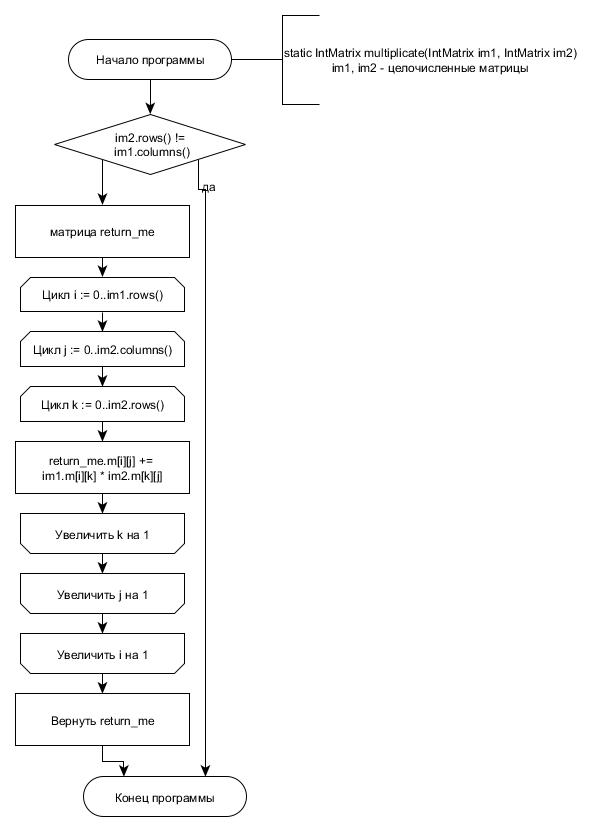
\includegraphics[scale=0.6]{classic.jpg}}
\caption{Функция классического умножения матриц.}
\label{ris:lev}
\end{figure}

\begin{figure}[pt!]
\center{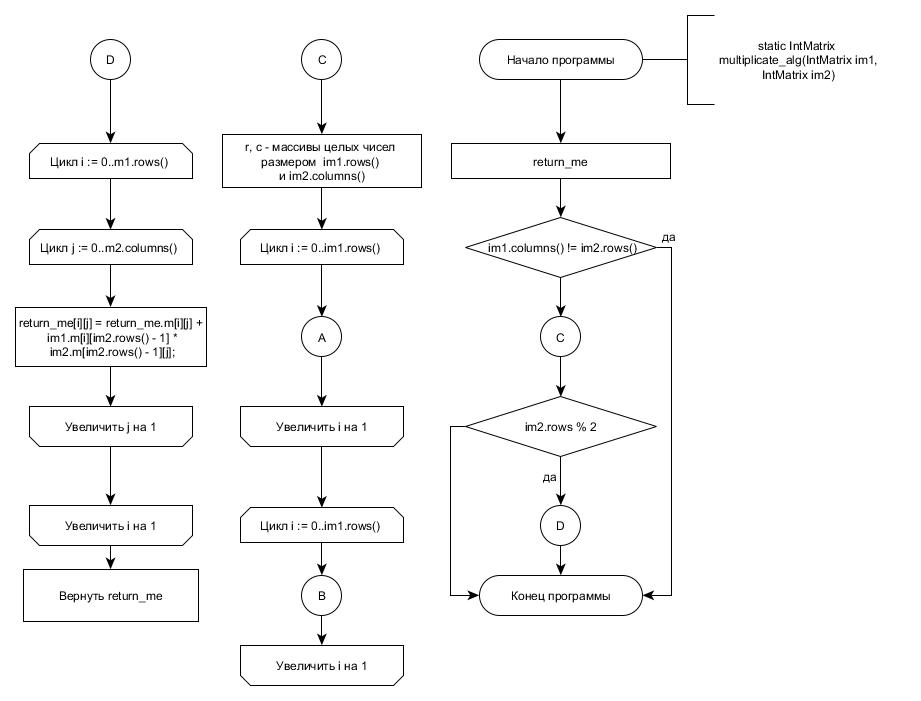
\includegraphics[scale=0.5]{vinograd.jpg}}
\caption{Функция алгоритма Винограда, часть 1}
\label{ris:dam_lev}
\end{figure}

\begin{figure}[pt!]
\center{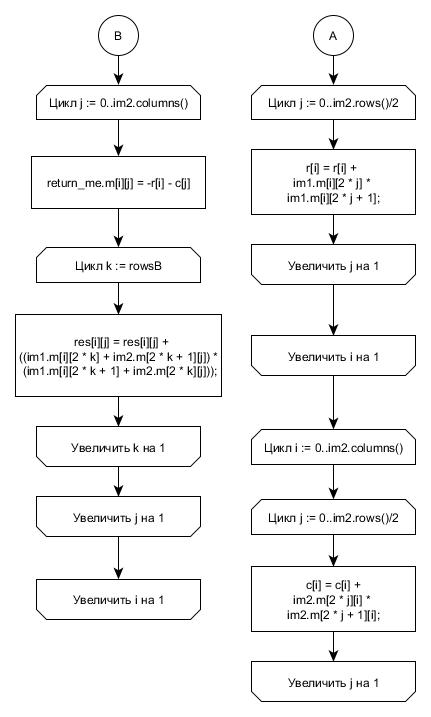
\includegraphics[scale=0.6]{vinograd2.jpg}}
\caption{Функция алгоритма Винограда, часть 2}
\label{ris:dam_lev}
\end{figure}

\begin{figure}[pt!]
\center{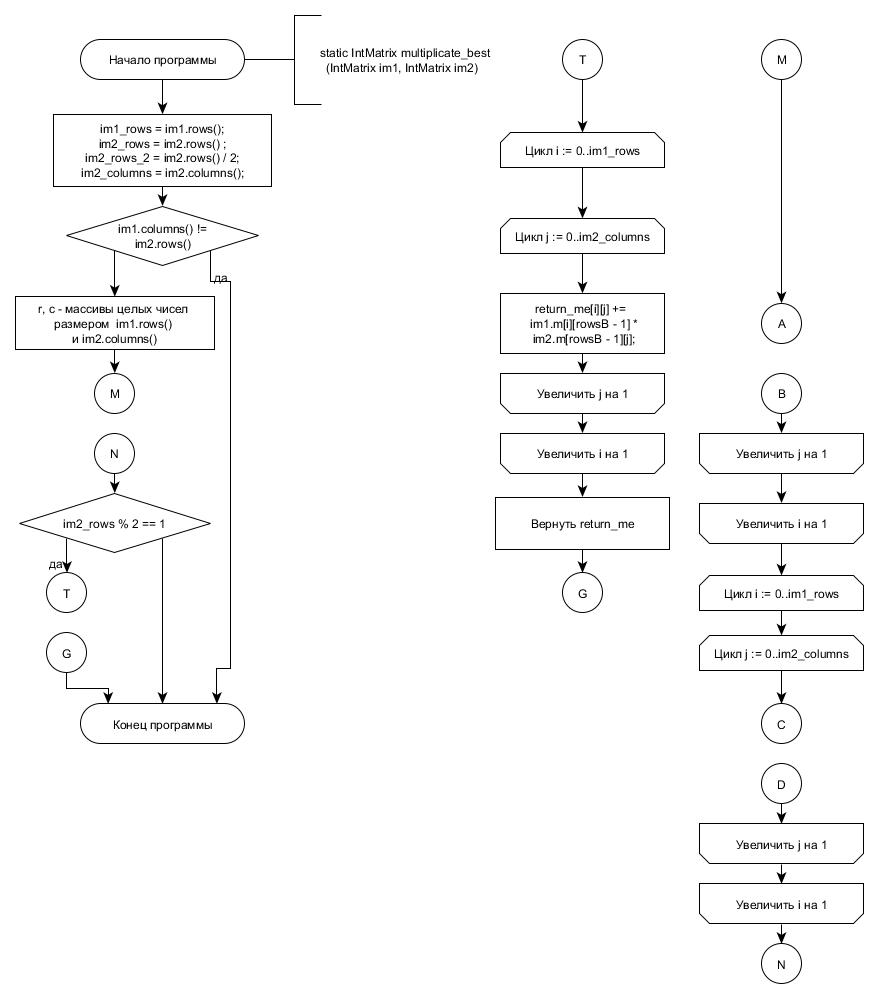
\includegraphics[scale=0.5]{vinograd_opt.jpg}}
\caption{Функция алгоритма Винограда с оптимизациями, часть 1}
\label{ris:dam_lev}
\end{figure}

\begin{figure}[pt!]
\center{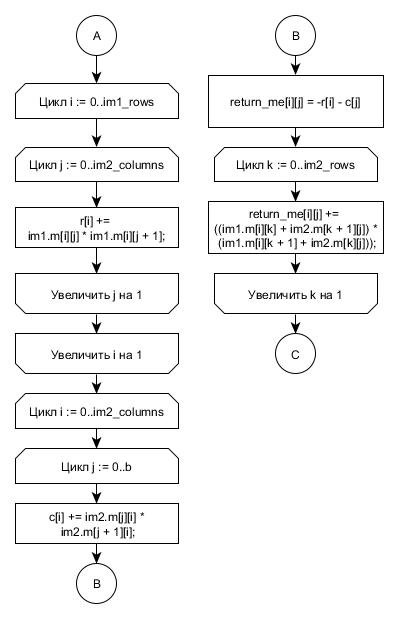
\includegraphics[scale=0.6]{vinograd_opt2.jpg}}
\caption{Функция алгоритма Винограда с оптимизациями, часть 2}
\label{ris:dam_lev}
\end{figure}
	
	\newpage
	\section{Технологическая часть}
	В данном разделе будут приведены требования к программнму обеспечению и средства реализации и листинг кода
	\subsection{Требования к программному обеспечению}
	 Требуется вводить две целочисленные матрицы и возвращать целочисленную матрицу - результат умножения. Допускается предоставление двух версий (либо режимов) ПО: для единичного эксперимента и для массовых экспериментов.
	\subsection{Средства реализации}
	Для реализации программ я выбрал язык программирования - C, так имею большой опыт работы с ним. Среда разработки - Qt. Для отключения оптимизации используется директива препроцессора - #pragma optimize("", off). Замеряется время работы процессора с помощью функции:\\
	\lstset{ %
        language=C++,                 % выбор языка для подсветки (здесь это С)
        basicstyle=\small\sffamily, % размер и начертание шрифта для подсветки кода
        numbers=left,               % где поставить нумерацию строк (слева\справа)
        numberstyle=\tiny,           % размер шрифта для номеров строк
        stepnumber=1,                   % размер шага между двумя номерами строк
        numbersep=-5pt,                % как далеко отстоят номера строк от         подсвечиваемого кода
        backgroundcolor=\color{white}, % цвет фона подсветки - используем         \usepackage{color}
        showspaces=false,            % показывать или нет пробелы специальными     отступами
        showstringspaces=false,      % показывать или нет пробелы в строках
        showtabs=false,             % показывать или нет табуляцию в строках
        frame=single,              % рисовать рамку вокруг кода
        tabsize=2,                 % размер табуляции по умолчанию равен 2 пробелам
        captionpos=t,              % позиция заголовка вверху [t] или внизу [b] 
        breaklines=true,           % автоматически переносить строки (да\нет)
        breakatwhitespace=false, % переносить строки только если есть пробел
        escapeinside={\%*}{*)},   % если нужно добавить комментарии в коде
	    keywordstyle=\color{blue}\ttfamily,
	    stringstyle=\color{red}\ttfamily,
	    commentstyle=\color{green}\ttfamily,
	    morecomment=[l][\color{magenta}]{\#},
	    columns=fullflexible
    }
	\begin{lstlisting}[label=time,caption=Функция замера процессороного времени]
    unsigned long long tick(void)
    {
        unsigned long long d;
        __asm__ __volatile__ ("rdtsc" : "=A"     (d));
        return d;
    }
	\end{lstlisting}
	Эта функция в отличие от встроенной функции таймера, способна считать реальное процессорное время работы программы в тиках\cite{lom}.

	\newpage
	\subsection{Реализация алгоритмов}
	
	\begin{lstlisting}[label=matrix-lev,caption=Классическая реализация умножения матриц]
   #pragma optimize("", off)
    static IntMatrix multiplicate(IntMatrix im1, IntMatrix im2) {
       if (im2.rows() != im1.columns())
            return (IntMatrix());
        IntMatrix return_me(im1.rows(), im2.columns());
        for (size_t i = 0; i < im1.rows(); i++) {// 3 + im1.rows()*(
            std::vector<int> row;
            return_me.m[i].clear(); //4 +
            for (size_t j = 0; j < im2.columns(); j++) {//3 + im2.columns()*(
                return_me.m[i].push_back(0); //4 +
                for (size_t k = 0; k < im2.rows(); k++) //3 + im2.rows() * (
                    return_me.m[i][j] = return_me.m[i][j] + im1.m[i][k] * im2.m[k][j]; // 15)))
            }
        }
        // 3 + im1.rows()*(4 + 3 + im2.columns()*(4 + 3 + im2.rows() * 12))

        // 3 + 7 * im1.rows() + 7 * im1.rows() * im2.columns() +
        // 12 * im1.rows() * im2.columns() * im2.rows()
        return return_me;
    }
	\end{lstlisting}
	
	\newpage
	\begin{lstlisting}[label=recur-lev,caption=Алгоритм Виноградова]
#pragma optimize("", off)
   static IntMatrix multiplicate_alg(IntMatrix im1, IntMatrix im2) {

        if (im2.rows() != im1.columns())
            return (IntMatrix());
        IntMatrix return_me(im1.rows(), im2.columns());

        std::vector<int> r(im1.rows());
        std::vector<int> c(im2.columns());

        for (size_t i = 0; i < im1.rows(); i++) { // 3 + im1.rows() * (
            for (size_t j = 0; j < im2.rows() / 2; j++) { //4 + im2.rows() *
                r[i] = r[i] + im1.m[i][2 * j] * im1.m[i][2 * j + 1]; //14)
            }
        }

        for (size_t i = 0; i < im2.columns(); i++) { // 3 + im2.columns() * (
            for (size_t j = 0; j < im2.rows() / 2; j++) {// 4 + im2.rows() *
                c[i] = c[i] + im2.m[2 * j][i] * im2.m[2 * j + 1][i]; //14)
            }
        }

        for (size_t i = 0; i < im1.rows(); i++) { // 3 + im1.rows() * (
            return_me.m[i].clear(); // 1 +
            for (size_t j = 0; j < im2.columns(); j++) { // 3 + im2.columns() * (
                return_me.m[i].push_back(0); // 3 +
                return_me.m[i][j] = -r[i] - c[j]; // 8 +
                for (size_t k = 0; k < im2.rows() / 2; k++) { // 4 + 1/2*im2.rows() *
                    return_me.m[i][j] =
                        return_me.m[i][j] + ((im1.m[i][2 * k] + im2.m[2 * k + 1][j]) *
                                             (im1.m[i][2 * k + 1] + im2.m[2 * k][j]));
                        //29))
                }
            }
        }

        if (im2.rows() % 2) { // 2 +
            for (size_t i = 0; i < im1.rows(); i++) { // 3 + im1.rows() * (
                for (size_t j = 0; j < im2.columns(); j++) { // 3 + im2.columns() *
                    return_me.m[i][j] = return_me.m[i][j] +
                        im1.m[i][im2.rows() - 1] * im2.m[im2.rows() - 1][j];
                    // 19)
                }
            }
        }

        //3 + im1.rows() * (4 + im2.rows() * 14) + 3 + im2.columns() * (4 + im2.rows() * 14) +
        //3 + im1.rows() * (4 + im2.columns() * (15 + im2.rows() * 29)) +
        //2 + 3 + im1.rows() * (3 + im2.columns() * 19)

        //14 + 11 * im1.rows() + 14 * im1.rows() * im2.rows() + 4 * im2.columns() + 14 * im2.columns() * im2.rows() +
        //im1.rows() * im2.columns() * 34 + 15 * im1.rows() * im2.columns() * im2.rows()

        return return_me;
    }
	\end{lstlisting}
	
	\newpage
	\begin{lstlisting}[label=matrix-lev,caption=Алгоритм Виноградова с оптимизациями]
  #pragma optimize("", off)
      static IntMatrix multiplicate_best(IntMatrix im1, IntMatrix im2) {

        if (im2.rows() != im1.columns())
            return (IntMatrix());
        IntMatrix return_me(im1.rows(), im2.columns());

        std::vector<int> r(im1.rows());
        std::vector<int> c(im2.columns());

        size_t im1_rows = im1.rows(); // 2 +
        size_t im2_rows_2 = im2.rows() / 2; // 3 +
        size_t im2_columns = im2.columns(); // 2 +

        for (size_t i = 0; i < im1_rows; i++) { // 2 + im1_rows * (
            for (size_t j = 0; j < im2_rows_2; j++) { // 2 + im2_rows_2 *
                r[i] += im1.m[i][j] * im1.m[i][j + 1]; // 10
            }
        }

        for (size_t i = 0; i < im2_columns; i++) { // 2 + im2_columns * (
            for (size_t j = 0; j < im2_rows_2; j++) { // 2 + im2_rows_2 * (
                c[i] += im2.m[j][i] * im2.m[j + 1][i]; // 10
            }
        }

        for (size_t i = 0; i < im1_rows; i++) { // 2 + im1_rows * (
            return_me.m[i].clear(); // 1 +
            for (size_t j = 0; j < im2_columns; j++) { // 2 + im2_columns * (
                return_me.m[i].push_back(0); // 3 +
                return_me.m[i][j] = -r[i] - c[j]; // 7 +
                for (size_t k = 0; k < im2_rows_2; k++) { //2 + im2_rows_2 *
                    return_me.m[i][j] += ((im1.m[i][k] + im2.m[k + 1][j]) *
                                          (im1.m[i][k + 1] + im2.m[k][j]));
                    // 21))
                }
            }
        }

        size_t im2_rows = im2.rows(); // 1 +
        if (im2_rows % 2) { // 1 +
            for (size_t i = 0; i < im1_rows; i++) { // 2 + im1_rows * (
                for (size_t j = 0; j < im2_columns; j++) {// 2 + im2_columns *
                    return_me.m[i][j] += im1.m[i][im2_rows - 1] * im2.m[im2_rows - 1][j];
                    // 13)
                }
            }
        }
        //7 +
        //2 + im1.rows() * (2 + im2.rows() * 10) + 2 + im2.columns() * (2 + im2.rows() * 10) +
        //2 + im1.rows() * (3 + im2.columns() * (12 + im2.rows() * 21)) +
        //4 + im1.rows() * (2 + im2.columns() * 13)

        //17 + 4 * im1.rows() + 10 * im1.rows() * im2.rows() + 2 * im2.columns() + 10 * im2.columns() * im2.rows() +
        //im1.rows() * im2.columns() * 16 + 21/2 * im1.rows() * im2.columns() * im2.rows()

        return return_me;
    }
	\end{lstlisting}
	
	
	


    \newpage
	\section{Экспериментальная часть}
	\hspace{1cm}В данном разделе будут приведены примеры работы программы, постановка эксперимента и сравнительный анализ алгоритмов на основе экспериментальных данных.
	\subsection{Примеры работы}
	\textbf {Пример 1}\\
	Матрица A = \\
	1 2 3\\
    4 5 6\\
    
    Матрица B = \\
	0 1 0 1\\
    1 0 1 0\\
    0 1 0 1\\
    
    Матрица A*B = \\
	2 4  2 4\\
    5 10 5 10\\\\
    \textbf {Пример 2}\\
	Матрица A = \\
	1 0\\
    2 0\\
    Матрица B = \\
	0 2\\
    0 1\\
    Матрица A*B = \\
	0 2\\
    0 4\\
    
    \newpage
    \textbf {Пример 3}\\
	Матрица A = \\
	10 -6\\
    Матрица B = \\
	6 5 4\\
    7 5 3\\
    Матрица A*B = \\
	18 20 22\\

    
    \subsection{Постановка эксперимента}
    \hspace{1cm}Для экспериментов использовались матрицы, размер которых варьируется от 100 до 800 с шагом 100 в случае чётной совпадающей размерности матриц (количества столбцов первой матрицы и количества строк второй матрицы) и от 101 до 801 с шагом 100 в случае нечётной размерности. 
    Количество повторов каждого эксперимента = 100. Результат одного эксперимента рассчитывается как
    средний из результатов проведенных испытаний с одинаковыми входными данными.
    
    
    \subsection{Сравнительный анализ на материале экспериментальных данных}
    В данном разделе будет проведен сравнительный анализ алгоритмов.
    \newpage
    \begin{table}
        \caption{\begin{center}
         \hspace{1cm}Результаты замеров времени, затрачиваемого классическим алгоритмом, алгоритмом винограда и улучшенным алгоритмом винограда для четных значений размеров матриц
        \end{center}}
        \begin{center}
            \begin{tabular}{ | c | c | c | c | }
                \hline
                 Количество элементов   &   Классический(ticks)   &   Виноград(ticks)  &  Виноград-улучшенный(tickes)\\ \hline  
                      100  &     63270859  &    61219632  &    46102778\\
                      200  &    576453831  &   510421544  &   357128872\\
                      300  &   1694622311  &  1572230360  &  1169622736\\
                      400  &   3921054927  &  3797844135  &  2800213561\\
                      500  &   7657814369  &  7865203454  &  6173433157\\
                      600  &  14940552478 &  14136962598  &  9698600460\\
                      700  &  22727058529 &  22511089261 &  15536365037\\
                      800  &  38324654343 &  36743546434 &  23453467743\\
                \hline
            \end{tabular}
        \end{center}
    \end{table}
    
    \begin{table}
        \caption{\begin{center}
         \hspace{1cm}Результаты замеров времени, затрачиваемого классическим алгоритмом, алгоритмом винограда и улучшенным алгоритмом винограда для нечетных значений размеров матриц
        \end{center}}
        \begin{center}
            \begin{tabular}{ | c | c | c | c | }
                \hline
                 Количество элементов   &   Классический(ticks)   &   Виноград(ticks)  &  Виноград-улучшенный(ticks)\\ \hline  
                       101  &    88123313  &    67439307  &    48911010\\
201  &    464202007  &   464567045  &   380656415\\
301  &   1800119731  &  1835463782  &  1502925015\\
401  &   4210485629  &  3759982040  &  2764641382\\
501  &   9841817407  & 11446977486  &  6927477537\\
601  &  16952357229 &  20596394054  & 13486175564\\
701  &  35802327580 &  24907672923 &  18292199385\\
801  &  42336980283 &  41194842838 &  28441949180\\
                \hline
            \end{tabular}
        \end{center}
    \end{table}
    
   \begin{center}График сравнения времени, затрачиваемого классическим алгоритмом, алгоритмом винограда и улучшенным алгоритмом винограда для четных значений размеров матриц\end{center}
    
    \begin{tikzpicture}
		\begin{axis}[
		    %title = График сравнения итеративной реализациии алгоритма Левенштейна и Дамерау-Левенштейна,
		    xlabel={Размерность матрицы},
		    ylabel={Время в тиках},
		    ymin = 0, ymax = 20542096398,
		    legend pos=north west,
		    ymajorgrids=true,
		    grid style=dashed,
		]
		
		
		\legend{ 
	        Классический, 
	        Виноград, 
	        Виноград улучшенный
	        }
  		\addplot[
  		    color=red,
  		    mark=square,
  		    ]
  		   coordinates {
  		    (100,63270859)
  		    (200,576453831)
  		    (300,1694622311)
  		    (400,3921054927)
			(500,7657814369)
			(600,14940552478)
			(700,22727058529)
			(800,38324654343)
  		    };

		\addplot[
  		    color=blue,
  		    mark=square,
  		    ]
  		    coordinates {
  		    (100,61219632)
  		    (200,510421544)
  		    (300,1572230360)
  		    (400,3797844135)
			(500,7865203454)
			(600,14136962598)
			(700,22511089261)
			(800,36743546434)
  		    };
  		    
  	    \addplot[
  		    color=green,
  		    mark=square,
  		    ]
  		    coordinates {
  		    (100,46102778)
  		    (200,357128872)
  		    (300,1169622736)
  		    (400,2800213561)
			(500,6173433157)
			(600,9698600460)
			(700,15536365037)
			(800,23453467743)
  		    };

		\end{axis}
	\end{tikzpicture}
	\newpage
	\begin{center}График сравнения времени, затрачиваемого классическим алгоритмом, алгоритмом винограда и улучшенным алгоритмом винограда для нечетных значений размеров матриц\end{center}
    
    \begin{tikzpicture}
		\begin{axis}[
		    %title = График сравнения итеративной реализациии алгоритма Левенштейна и Дамерау-Левенштейна,
		    xlabel={Размерность матрицы},
		    ylabel={Время в тиках},
		    ymin = 0, ymax = 21842065660,
		    legend pos=north west,
		    ymajorgrids=true,
		    grid style=dashed,
		]
		
		
		\legend{ 
	        Классический, 
	        Виноград, 
	        Виноград улучшенный
	        }
  		\addplot[
  		    color=red,
  		    mark=square,
  		    ]
  		    coordinates {
  		    (101,88123313)
  		    (201,464202007)
  		    (301,1800119731)
  		    (401,4210485629)
			(501,9841817407)
			(601,16952357229)
			(701,35802327580)
			(801,42336980283)
  		    };

		\addplot[
  		    color=blue,
  		    mark=square,
  		    ]
  		    coordinates {
  		    (101,67439307)
  		    (201,464567045)
  		    (301,1835463782)
  		    (401,3759982040)
			(501,11446977486)
			(601,20596394054)
			(701,24907672923)
			(801,41194842838)
  		    };
  		    
  		\addplot[
  		    color=green,
  		    mark=square,
  		    ]
  		    coordinates {
  		    (101,48911010)
  		    (201,380656415)
  		    (301,1502925015)
  		    (401,2764641382)
			(501,6927477537)
			(601,13486175564)
			(701,18292199385)
			(801,28441949180)
  		    };

		\end{axis}
	\end{tikzpicture}
	
    \newpage
	\section*{Вывод}
    \addcontentsline{toc}{section}{Вывод}
    
    
	\hspace{1cm}В результате проведенного эксперимента был получен следующий вывод: алгоритм Винограда в своем изначальном виде незначительно быстрее классического алгоритма, однако после применения оптимизаций, алгоритм Винограда становится примерно в 2 раза быстрее классического алгоритма. Этот отрыв сокращается незначительно при умножении матриц нечетных размерностей. Сложность стандартного алгоритма 
	\newpage
	\section*{Заключение}
    \addcontentsline{toc}{section}{Заключение}
    
	\hspace{1cm}В ходе работы были изучены и реализованы алгоритмы классического умножения матриц , алгоритма Виноградова и алгоритма Виноградова с оптимизациями. Также был проведен сравнительный анализ перечисленных алгоритмов.. Экспериментально подтверждено различие во временнoй эффективности. Классический алгоритм работает медленнее, чем алгоритм Винограда или его оптимизированная версия, поскольку если обычный алгоритм работает за 13*n3 (с учетом, что на вход пришли две квадратных матрицы размера n), то алгоритм Винограда работает за 13n3, а его улучшенная версия 9*n3. При этом с точки зрения объема затрачиваемой памяти, он более эффективен, поскольку не выделяет память под дополнительные массивы, как это делает алгоритм Винограда. Если же говорить об обычном и оптимизированным, то оптимизированный работает быстрее за счет занесения вычисления B/2 в отдельную переменную и измененный пересчет вспомогательных строк r и c.
    

    \newpage

    \addcontentsline{toc}{section}{Список литературы}
    \begin{thebibliography}{9} 
    \bibitem{lev_1} Henry Cohn, Robert Kleinberg, Balazs Szegedy, and Chris Umans. Group-theoretic Algorithms for Matrix Multiplication. arXiv:math.GR/0511460. Proceedings of the 46th Annual Symposium on Foundations of Computer Science, 23-25 October 2005, Pittsburgh, PA, IEEE Computer Society, pp. 379—388.. 
    \bibitem{lev_2} Don Coppersmith and Shmuel Winograd. Matrix multiplication via arithmetic progressions. Journal of Symbolic Computation, 9:251-280, 1990.
    \bibitem{lom}И.В. Ломовской. Курс лекций по языку программирования C, 2017
    
    \end{thebibliography}

		
		
		
\end{document}